\chapter{LAPORAN}
\section{Teori}
\subsection{Kecerdasan Buatan}
\begin{enumerate}
    \item Definisi\\
    Kecerdasan buatan atau Artificial Intelligence merupakan suatu bentuk tiruan atau simulasi dari kecerdasan manusia yang kemudian dimodelkan dalam mesin seperti komputer dan kemudian diprogram sedemikian rupa sehingga dapat memiliki cara kerja/pikir seperti pada manusia.
    \item Sejarah dan Perkembangan\\
    Sejak awal kemunculan komputer pada sekitar tahun 1940, telah difokuskan pengerjaan sesuatu yang biasa dilakukan manusia untuk dialihkan ke komputer, sehingga komputer dapat menirukan serta melakukan kecerdasan dan perilaku seperti yang dilakukan oleh manusia.\\
    \par
    Pada tahun 1945, McMullo dan Pitts mengusulkan sebuah model matematis yang dinamakan perceptron dari neuron dari otak yang menunjukkan bagaimana neuron dapat aktif seperti halnya sakar yang adat dihidupkan maupun dimatikan, serta dapat belajar dan memberi aksi yang berbeda terhadap waktu tiap input yang diberikan.
    Kemudian pada tahun 1950, diadakan sebuah research mengenai kecerdasan buatan pada paper Alan Turing dengan judul "Computing Machineri and Intelligence" yang mendiskusikan syarat mesin dapat dianggap cerdas, yaitu apabila medin tersebut dapat berperilaku seperti manusia dengan sukses.
    \par 
    Pada akhir tahun 1955, dikembangkannya The Logic Theprist oleh Newell dan Simon sebagai program kecerdasan pertama kali, program ini menjelaskan berbagai masalah dengan decision tree dan menyelesaikannya dengan memilih cabang yang menghasilkan kesimpulan akhir paling benar.\\
    Setelahnya, pada tahun 1956, John McChary dari Massacuhetts Institute of Technology dijuluki sebagai bapak AI, beliau menyelenggarakan suatu konferensi yang ditujukan untuk menarik para ahli komputer bertemu, konferensi tersebut dinamakan "The Dartmouth summer research project on artificial intelligence".
\end{enumerate}
\subsection{Pengertian Istilah}
\begin{enumerate}
\item Supervised Learning\\
Supervised learning merupakan suatu algoritma yang digunakan untuk menentukan suatu prediksi dan klasifikasi berdasarkan variabel x dan variabel y telah diketahui. Algoritma ini seolah-olah sudah dilatih sehingga dapat menghasilkan suatu bentuk prediksi dan klasifikasi
    \item Klasifikasi\\
    Klasifikasi yaitu pengelompokan suatu hal berdasarkan kelas, persamaan maupun perbedaan yang ada.
    \item Regresi\\
    Regresi ialah suatu metode statistik yang digunakan untuk menentukan karakter maupun relasi dari suatu variabel dependen terhadap variabel yang lainnya.
    \item Unsupervised learning\\
    Unsupervised learning yaitu suatu algoritma penentuan prediksi dimana data tidak memiliki output/target variablenya, sehingga tidak yang mengendalikan jalannya algoritma suatu program. Berbeda dengan supervised learning, algoritma ini tidak perlu dilatih dahulu untuk dapat mengjasilkan prediksi maupun klasifikasi.
    \item Data set\\
    Dataset merupakan kumpulan data yang kemudian akan diinputkan dalam program dan diproses. Dataset dapat berupa point, record, vektor, case, pattern, dan sebagainya.
    \item Training set\\
    Training set ialah suatu bagian dari datasey yang dilatih untuk dapat membuat suatu prediksi dan klasifikasi.
    \item Testing set\\
    Testing set merupakan suatu bagian dataset yang akan diuji, testing ditujukan untuk mengukur seberapa akurat hasil prediksi dari data tersebut.\\
\end{enumerate}
\section{Instalasi}
\begin{enumerate}
    \item Instalasi Library scikit-learn
    \begin{figure}[H]
    \centering
    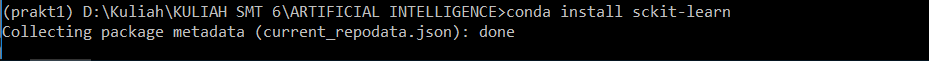
\includegraphics[width=1\textwidth]{figures/1184030/Screenshot (2143).png}
    \caption{Instalasi Library Scikit-Learn}
    \label{fig:my_label}
\end{figure}
\begin{figure}[H]
    \centering
    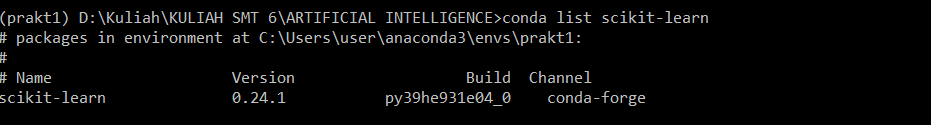
\includegraphics[width=1\textwidth]{figures/1184030/Screenshot (2144).png}
    \caption{Cek Apakah Library Scikit-Learn sudah terinstall}
    \label{fig:my_label}
\end{figure}
    \item Mencoba Loading an example dataset, menjelaskan maksud dari tulisan tersebut dan mengartikan per baris.\\
Loading an example dataset (memuat contoh kumpulan data) maksudnya yaitu scikit-learn memugkinkan kita untuk mengambil atau memuat data standar, misalnya kita mengambil atau memuat data set iris dan digits untuk membuat sebuah klasifikasi dan data set diabetes untuk regresi.\\
\begin{figure}[H]
    \centering
    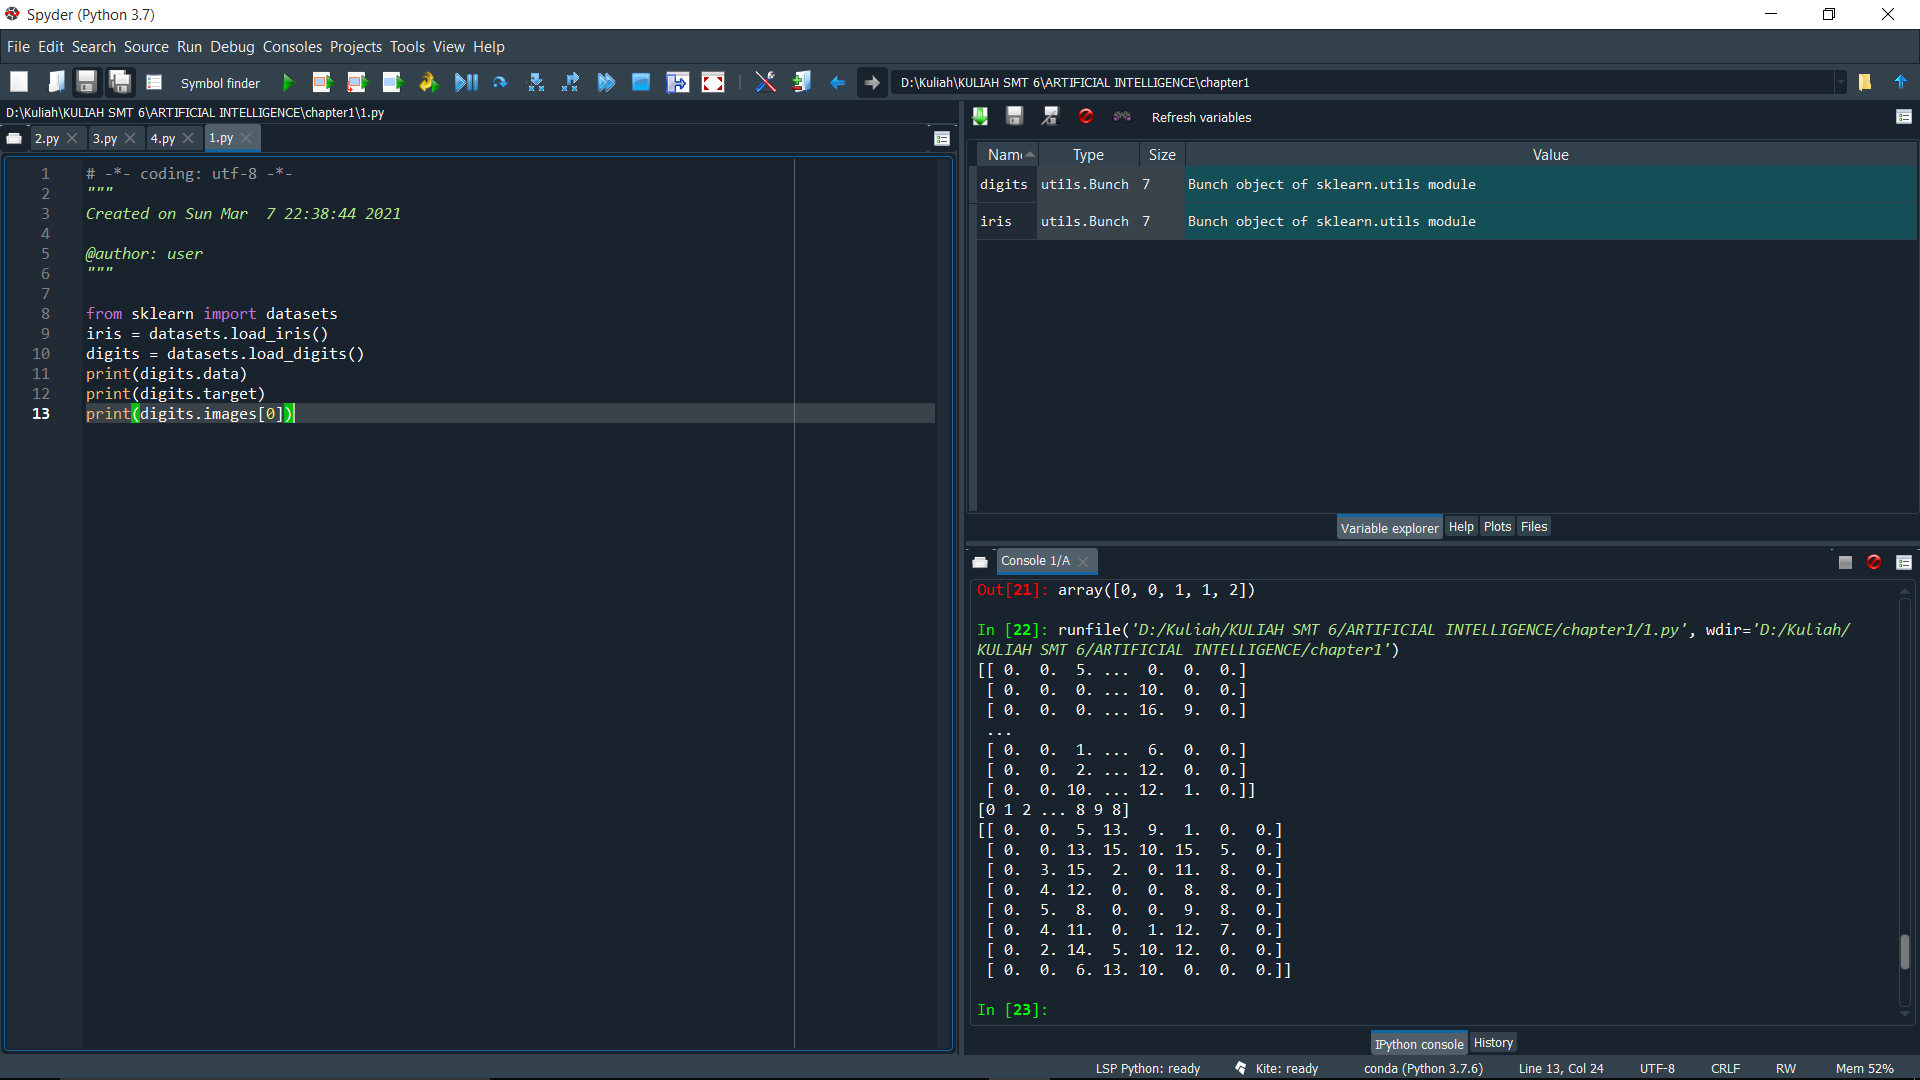
\includegraphics[width=1\textwidth]{figures/1184030/Screenshot (2159).png}
    \caption{Loading an example}
    \label{fig:my_label}
\end{figure}
\begin{lstlisting}
from sklearn import datasets
iris = datasets.load_iris()
digits = datasets.load_digits()
#print(digits.data)
#print(digits.target)
print(digits.images[0])
\end{lstlisting}
Berikut ini penjelasan perbarisnya :\\
\begin{itemize}
    \item from sklearn import datasets\\
    mengimportkan dataset dari library sklearn
    \item iris = datasets.load\_iris()\\
    mendefinisikan variable iris dengan menggunakan load\_iris() dari dataset yang telah diimport sebelumnya
    \item digits = datasets.load\_digits()\\
     mendefinisikan variable digits dengan menggunakan load\_digits() dari dataset yang telah diimport sebelumnya
    \item print(digits.data)\\
    mencetak isi dari variable digits
    \item print(digits.target)\\
    mencetak array target yang sesuai dari variable digits
    \item print(digits.images[0])
\end{itemize}
\item 
Mencoba Learning and predicting, menjelaskan maksud dari tulisan tersebut dan mengartikan per baris.\\

Learning and Predicting (Belajar dan Memprediksi) maksudnya yaitu belajar dari sebuah model dan membuatkan prediksi dalam sebuah gambar. Menggunakan data set digits karena data digits dapat memprediksi, mengingat gambar digit mana yang diwakilinya. \\

\begin{lstlisting}
#learning and predicting
from sklearn import svm
clf = svm.SVC(gamma=0.001, C=100.)
x = clf.fit(digits.data[:-1], digits.target[:-1]) #fit x,y
print(x)
y = clf.predict(digits.data[-1:]) #y = hasil prediksi data baru
print(y)
\end{lstlisting}
berikut ini penjelasan perbarisnya, yaitu :\\
\begin{itemize}
    \item from sklearn import svm\\
    mengimportkan svm pada library sklearn
    \item clf = svm.SVC(gamma=0.001, C=100.)\\
    mendefinisikan variable slf dengan mengambil function SVC dari svm yang telah diimport sebelumnya
    \item x = clf.fit(digits.data[:-1], digits.target[:-1]) \\
    fit x,y
    \item y = clf.predict(digits.data[-1:])\\
mendefinisikan hasil prediksi data baru
\end{itemize}
\item 
mencoba Model persistence, menjelaskan maksud dari tulisan tersebut dan mengartikan per baris.\\
Model Presistence maksudnya mempertahankan sebuah model agar bisa digunakan di masa depan tanpa perlu melatih kembali atau membuat model itu kembali. Menyimpan model dengan menggunakan pickle atau joblib
\begin{lstlisting}
from sklearn import svm
from sklearn import datasets
clf = svm.SVC()
X, y = datasets.load_iris(return_X_y=True)
clf.fit(X, y)
#contoh menggunakan pickle
import pickle
a = pickle.dumps(clf)
clf2 = pickle.loads(a)
clf2.predict(X[0:1])
y[0]
\end{lstlisting}
\item 
Mencoba Conventions, menjelaskan maksud dari tulisan tersebut dan mengartikan per baris.\\

Conventions (konvensi) maksudnya dapat memprediksi dengan lebih prediktif.\\
\begin{itemize}
    \item Type casting
    \begin{lstlisting}
#conventions type casting
import numpy
from sklearn import random_projection
rng = numpy.random.RandomState(0)
X = rng.rand(10, 2000)
X =numpy.array(X, dtype='float32')
X.dtype #type floatnya 32
transformer = random_projection.GaussianRandomProjection()
X_new = transformer.fit_transform(X)
X_new.dtype #type floatnya 64 
    \end{lstlisting}
    \item Refitting and updating parameters
\begin{lstlisting}
#conventions refitting and updating parameters
import numpy as np #mengimportkan library numpy dan dialiaskan dengan np
from sklearn.datasets import load_iris #mengimportkan load_iris dari sklearn.datasets
from sklearn.svm import SVC #mengimportkan SVC dari sklearn.svm
X, y = load_iris(return_X_y=True)
clf = SVC()
clf.set_params(kernel='linear').fit(X, y)
clf.predict(X[:5])
clf.set_params(kernel='rbf').fit(X, y)
clf.predict(X[:5])
\end{lstlisting}
    \item multiclass vs multilabel fitting
\begin{lstlisting}
#multiclass
from sklearn.svm import SVC
from sklearn.multiclass import OneVsRestClassifier
from sklearn.preprocessing import LabelBinarizer
X = [[1, 2], [2, 4], [4, 5], [3, 2], [3, 1]]
y = [0, 0, 1, 1, 2]
classif = OneVsRestClassifier(estimator=SVC(random_state=0))
classif.fit(X, y).predict(X) #menghasilkan array 1 dimensi

#multiple labels

y = LabelBinarizer().fit_transform(y)
classif.fit(X, y).predict(X) #menghasilkan array 2 dimensi namun, hasil pada array ke 3 dan 4 bernilai 0

#pengklasifikasian array 2 dimensi dengan multilabel yang diprediksi pada tiap instance
from sklearn.preprocessing import MultiLabelBinarizer
y = [[0, 1], [0, 2], [1, 3], [0, 2, 3], [2, 4]]
y = MultiLabelBinarizer().fit_transform(y)
classif.fit(X, y).predict(X)
\end{lstlisting}
\end{itemize}
\end{enumerate}
\section{Penanganan Error}
\begin{enumerate}
	\item
	skrinsut error[hari ke 2](10)
	\item
Tuliskan kode eror dan jenis errornya [hari ke 2](10)
	\item
Solusi pemecahan masalah error tersebut[hari ke 2](10)

\end{enumerate}